\documentclass[12pt,a4paper,openany]{report}

% ─────────────────────────────────────────────
%  PACKAGES
% ─────────────────────────────────────────────
\usepackage[a4paper, top=26mm, bottom=26mm, left=28mm, right=24mm]{geometry}
\usepackage[T1]{fontenc}
\usepackage[utf8]{inputenc}
\usepackage{amsmath, amssymb}
\usepackage{graphicx}
\usepackage{xcolor}
\usepackage{tikz}
\usetikzlibrary{shapes.geometric, arrows.meta, positioning, calc, fit, backgrounds, decorations.pathreplacing}
\usepackage{tcolorbox}
\tcbuselibrary{skins, breakable}
\usepackage{listings}
\usepackage{booktabs}
\usepackage{array}
\usepackage{tabularx}
\usepackage{multirow}
\usepackage{hyperref}
\usepackage{fancyhdr}
\usepackage{titlesec}
\usepackage{titletoc}
\usepackage{enumitem}
\usepackage{mdframed}
\usepackage{setspace}
\usepackage{caption}
\usepackage{makecell}
\usepackage{colortbl}
\usepackage{longtable}
\usepackage{pmboxdraw}

% ─────────────────────────────────────────────
%  TERMINAL / HACKER COLOUR PALETTE
% ─────────────────────────────────────────────
\definecolor{TermBg}{RGB}{10, 14, 10}          % near-black bg
\definecolor{TermBgLight}{RGB}{16, 22, 16}     % slightly lighter
\definecolor{TermBgPanel}{RGB}{20, 30, 20}     % panel bg
\definecolor{TermGreen}{RGB}{0, 255, 70}       % bright green
\definecolor{TermGreenDim}{RGB}{0, 180, 50}    % dimmer green
\definecolor{TermGreenPale}{RGB}{0, 100, 30}   % very dim green
\definecolor{TermAmber}{RGB}{255, 176, 0}      % amber accent
\definecolor{TermCyan}{RGB}{0, 230, 220}       % cyan accent
\definecolor{TermRed}{RGB}{255, 60, 60}        % error red
\definecolor{TermWhite}{RGB}{200, 220, 200}    % off-white text
\definecolor{TermGray}{RGB}{80, 110, 80}       % dim text
\definecolor{TermDarkGray}{RGB}{35, 50, 35}    % separator lines
\definecolor{CodeKw}{RGB}{0, 255, 70}
\definecolor{CodeCmt}{RGB}{80, 160, 80}
\definecolor{CodeStr}{RGB}{255, 176, 0}
\definecolor{CodeNum}{RGB}{0, 220, 220}
\definecolor{CodePre}{RGB}{200, 100, 255}

% ─────────────────────────────────────────────
%  PAGE BACKGROUND
% ─────────────────────────────────────────────
\pagecolor{TermBg}
\color{TermWhite}

% ─────────────────────────────────────────────
%  HEADER / FOOTER
% ─────────────────────────────────────────────
\pagestyle{fancy}
\fancyhf{}
\renewcommand{\headrulewidth}{0pt}
\renewcommand{\footrulewidth}{0pt}
\fancyhead[L]{%
  \colorbox{TermBgPanel}{%
    \color{TermGreen}\ttfamily\small\bfseries
    \quad\textgreater\_\ \nouppercase{\leftmark}\quad}}
\fancyhead[R]{%
  \colorbox{TermBgPanel}{%
    \color{TermAmber}\ttfamily\small
    \quad mobile-embedded-dev\quad}}
\fancyfoot[C]{\color{TermGray}\ttfamily\small ---\ \thepage\ ---}
\fancyfoot[L]{\color{TermGray}\ttfamily\footnotesize \$ termux + neovim + arduinodroid}
\fancyfoot[R]{\color{TermGray}\ttfamily\footnotesize 2026}
\setlength{\headheight}{18pt}

% ─────────────────────────────────────────────
%  CHAPTER / SECTION HEADINGS
% ─────────────────────────────────────────────
\titleformat{\chapter}[display]
  {\normalfont\ttfamily\huge\bfseries\color{TermGreen}}
  {%
    \color{TermGray}\small\ttfamily
    [\,chapter\ \thechapter\,]
  }
  {4pt}
  {\color{TermGreen}\huge\bfseries\ttfamily}
  [\vspace{4pt}{\color{TermGreenPale}\rule{\linewidth}{1.2pt}}]
\titlespacing*{\chapter}{0pt}{-10pt}{18pt}

\titleformat{\section}
  {\color{TermAmber}\large\bfseries\ttfamily}
  {\color{TermGray}\ttfamily\S\thesection\enspace}
  {0pt}
  {}
  [\color{TermDarkGray}\vspace{2pt}\hrule\vspace{4pt}]

\titleformat{\subsection}
  {\color{TermCyan}\normalsize\bfseries\ttfamily}
  {\color{TermGray}\ttfamily\thesubsection\enspace}
  {0pt}
  {}

\titleformat{\subsubsection}
  {\color{TermGreenDim}\small\bfseries\ttfamily}
  {\color{TermGray}\ttfamily\thesubsubsection\enspace}
  {0pt}
  {}

% ─────────────────────────────────────────────
%  TOC STYLE
% ─────────────────────────────────────────────
\titlecontents{chapter}[0pt]
  {\vspace{4pt}\bfseries\ttfamily\color{TermGreen}}
  {\thecontentslabel\enspace}
  {}
  {\color{TermGray}\titlerule*[6pt]{.}\color{TermAmber}\contentspage}

\titlecontents{section}[1.6em]
  {\small\ttfamily\color{TermWhite}}
  {\thecontentslabel\enspace}
  {}
  {\color{TermGray}\titlerule*[5pt]{.}\color{TermGreenDim}\contentspage}

\titlecontents{subsection}[3.2em]
  {\footnotesize\ttfamily\color{TermGray}}
  {\thecontentslabel\enspace}
  {}
  {\color{TermGray}\titlerule*[5pt]{.}\contentspage}

% ─────────────────────────────────────────────
%  TCOLORBOX ENVIRONMENTS
% ─────────────────────────────────────────────
\newtcolorbox{termbox}[1][\$\ terminal]{
  enhanced, breakable, arc=0pt, boxrule=0pt,
  colback=TermBgPanel,
  borderline west={2pt}{0pt}{TermGreen},
  borderline north={0.4pt}{0pt}{TermGreenPale},
  borderline south={0.4pt}{0pt}{TermGreenPale},
  fonttitle=\ttfamily\bfseries\small\color{TermGreen},
  title={#1},
  left=10pt, right=10pt, top=7pt, bottom=7pt,
  coltitle=TermGreen
}

\newtcolorbox{notebox}[1][NOTE]{
  enhanced, breakable, arc=0pt, boxrule=0pt,
  colback=TermBgPanel,
  borderline west={2pt}{0pt}{TermCyan},
  fonttitle=\ttfamily\bfseries\small\color{TermCyan},
  title={[\,#1\,]},
  left=10pt, right=10pt, top=7pt, bottom=7pt,
}

\newtcolorbox{warnbox}[1][WARNING]{
  enhanced, breakable, arc=0pt, boxrule=0pt,
  colback=TermBgPanel,
  borderline west={2pt}{0pt}{TermRed},
  fonttitle=\ttfamily\bfseries\small\color{TermRed},
  title={[\,!\,]\ #1},
  left=10pt, right=10pt, top=7pt, bottom=7pt,
}

\newtcolorbox{tipbox}[1][TIP]{
  enhanced, breakable, arc=0pt, boxrule=0pt,
  colback=TermBgPanel,
  borderline west={2pt}{0pt}{TermAmber},
  fonttitle=\ttfamily\bfseries\small\color{TermAmber},
  title={[\,\#\,]\ #1},
  left=10pt, right=10pt, top=7pt, bottom=7pt,
}

\newtcolorbox{successbox}[1][OK]{
  enhanced, breakable, arc=0pt, boxrule=0pt,
  colback=TermBgPanel,
  borderline west={2pt}{0pt}{TermGreen},
  fonttitle=\ttfamily\bfseries\small\color{TermGreen},
  title={[\,\checkmark\,]\ #1},
  left=10pt, right=10pt, top=7pt, bottom=7pt,
}

% ─────────────────────────────────────────────
%  CODE LISTINGS
% ─────────────────────────────────────────────
\lstdefinestyle{terminal}{
  basicstyle=\ttfamily\small\color{TermGreen},
  backgroundcolor=\color{TermBgPanel},
  breaklines=true, frame=none,
  xleftmargin=14pt, numbers=none,
  showstringspaces=false,
}
\lstdefinestyle{shell}{
  basicstyle=\ttfamily\small\color{TermWhite},
  backgroundcolor=\color{TermBgPanel},
  keywordstyle=\color{TermGreen}\bfseries,
  commentstyle=\color{CodeCmt}\itshape,
  stringstyle=\color{CodeStr},
  breaklines=true, frame=none,
  xleftmargin=14pt, numbers=none,
  showstringspaces=false,
  morecomment=[l]{\#},
}
\lstdefinestyle{asmstyle}{
  basicstyle=\ttfamily\small\color{TermWhite},
  backgroundcolor=\color{TermBgPanel},
  keywordstyle=\color{CodeKw}\bfseries,
  commentstyle=\color{CodeCmt}\itshape,
  stringstyle=\color{CodeStr},
  numberstyle=\tiny\color{TermGray},
  numbers=left, numbersep=10pt,
  breaklines=true, frame=none,
  xleftmargin=24pt,
  showstringspaces=false,
  morecomment=[l]{;},
  morekeywords={ldi,out,rjmp,in,sbis,sbic,cbi,sbi,nop,ret,
                reti,push,pop,clr,ser,inc,dec,add,sub,and,
                or,eor,com,neg,cp,cpc,breq,brne,brcs,brcc,
                brsh,brlo,brmi,brpl,brtc,brts,brvc,brvs,
                brge,brlt,call,rcall,jmp,ld,st,ldd,std,
                lpm,spm,mov,movw,adc,sbc,mul,muls,mulsu,
                adiw,sbiw,andi,ori,sbr,cbr,tst,clc,sec,
                cli,sei,clt,set,clv,sev,cls,ses,cln,sen,
                clz,sez,clh,seh,wdr,sleep,break},
  morekeywords=[2]{.include,.org,.def,.equ,.cseg,.dseg,
                   .eseg,.db,.dw,.byte,.text,.data,
                   DDRB,DDRC,DDRD,PORTB,PORTC,PORTD,
                   PINB,PINC,PIND,SREG,SPH,SPL,
                   TCCR0A,TCCR0B,TCCR1A,TCCR1B,
                   TCNT0,TCNT1,OCR0A,OCR1A,TIMSK0,
                   TIMSK1,TIFR0,TIFR1,UCSR0A,UCSR0B,
                   UBRR0H,UBRR0L,UDR0},
  keywordstyle=[2]\color{CodePre}\bfseries,
}
\lstdefinestyle{cstyle}{
  language=C,
  basicstyle=\ttfamily\small\color{TermWhite},
  backgroundcolor=\color{TermBgPanel},
  keywordstyle=\color{CodeKw}\bfseries,
  commentstyle=\color{CodeCmt}\itshape,
  stringstyle=\color{CodeStr},
  numberstyle=\tiny\color{TermGray},
  numbers=left, numbersep=10pt,
  breaklines=true, frame=none,
  xleftmargin=24pt,
  showstringspaces=false,
  morecomment=[l]{//},
  morekeywords={pinMode,digitalWrite,digitalRead,
                delay,delayMicroseconds,
                OUTPUT,INPUT,INPUT_PULLUP,HIGH,LOW,
                uint8_t,uint16_t,uint32_t,
                void,int,bool,byte,word,long},
}
\lstset{style=shell}

% ─────────────────────────────────────────────
%  TABLE HELPERS
% ─────────────────────────────────────────────
\newcolumntype{L}[1]{>{\raggedright\arraybackslash}p{#1}}
\newcolumntype{C}[1]{>{\centering\arraybackslash}p{#1}}
\renewcommand{\arraystretch}{1.4}
\newcommand{\thdg}[1]{\cellcolor{TermBgPanel}\color{TermGreen}\ttfamily\bfseries #1}
\newcommand{\thda}[1]{\cellcolor{TermBgPanel}\color{TermAmber}\ttfamily\bfseries #1}
\newcommand{\altrow}{\rowcolor{TermBgPanel}}

% ─────────────────────────────────────────────
%  HYPERREF
% ─────────────────────────────────────────────
\hypersetup{
  colorlinks=true,
  linkcolor=TermGreen,
  urlcolor=TermCyan,
  citecolor=TermAmber,
  pdftitle={Mobile Embedded Dev Guide}
}

\setlength{\parskip}{5pt}
\setlength{\parindent}{0pt}
\captionsetup{
  font=small,
  labelfont={bf},
  labelsep=period,
  textfont={color=TermWhite},
  labelfont={color=TermGreen,bf,tt}
}

% ════════════════════════════════════════════════════════
\begin{document}
\pagecolor{TermBg}   % <-- here, not in preamble
\color{TermWhite}

% ─────────────────────────────────────────────
%  COVER PAGE
% ─────────────────────────────────────────────
\begin{titlepage}
\thispagestyle{empty}
\pagecolor{TermBg}


\begin{tikzpicture}[remember picture, overlay]
  % Scanline effect strips
  \foreach \y in {0,0.4,...,30} {
    \fill[TermGreen, opacity=0.012]
      (current page.south west) ++(0,\y cm)
      rectangle +(\paperwidth, 0.18cm);
  }
  % Corner brackets
  \draw[TermGreen, line width=1.2pt]
    ([xshift=1.2cm, yshift=-1.2cm]current page.north west) --
    ([xshift=1.2cm, yshift=-2.6cm]current page.north west);
  \draw[TermGreen, line width=1.2pt]
    ([xshift=1.2cm, yshift=-1.2cm]current page.north west) --
    ([xshift=2.8cm, yshift=-1.2cm]current page.north west);
  \draw[TermGreen, line width=1.2pt]
    ([xshift=-1.2cm, yshift=-1.2cm]current page.north east) --
    ([xshift=-1.2cm, yshift=-2.6cm]current page.north east);
  \draw[TermGreen, line width=1.2pt]
    ([xshift=-1.2cm, yshift=-1.2cm]current page.north east) --
    ([xshift=-2.8cm, yshift=-1.2cm]current page.north east);
  \draw[TermGreen, line width=1.2pt]
    ([xshift=1.2cm, yshift=1.2cm]current page.south west) --
    ([xshift=1.2cm, yshift=2.6cm]current page.south west);
  \draw[TermGreen, line width=1.2pt]
    ([xshift=1.2cm, yshift=1.2cm]current page.south west) --
    ([xshift=2.8cm, yshift=1.2cm]current page.south west);
  \draw[TermGreen, line width=1.2pt]
    ([xshift=-1.2cm, yshift=1.2cm]current page.south east) --
    ([xshift=-1.2cm, yshift=2.6cm]current page.south east);
  \draw[TermGreen, line width=1.2pt]
    ([xshift=-1.2cm, yshift=1.2cm]current page.south east) --
    ([xshift=-2.8cm, yshift=1.2cm]current page.south east);
  % Vertical left stripe
  \fill[TermGreenPale]
    ([xshift=0cm]current page.south west)
    rectangle ([xshift=0.35cm]current page.north west);
  \fill[TermGreen]
    ([xshift=0cm]current page.south west)
    rectangle ([xshift=0.12cm]current page.north west);
\end{tikzpicture}

\vspace*{2.0cm}
\hspace{1.5cm}
%\begin{minipage}{\dimexpr\linewidth - 2.0cm}

{\color{TermGray}\ttfamily\footnotesize
\textgreater\ initializing documentation system...\ [OK]\\
\textgreater\ loading workflow modules...\ [OK]\\
\textgreater\ rendering cover page...\ [OK]\\[18pt]}

{\color{TermGreen}\ttfamily\fontsize{9}{11}\selectfont
\# ══════════════════════════════════════════════ \#}\\[6pt]

{\color{TermGreen}\ttfamily\fontsize{36}{42}\selectfont\bfseries
Arduino and Assembly Files }\\[2pt]
{\color{TermGreen}\ttfamily\fontsize{25}{42}\selectfont\bfseries
Using Termux and ArduinoDroid}\\[10pt]

{\color{TermAmber}\ttfamily\Large
Termux\ +\ Neovim\ +\ AVR\ +\ ArduinoDroid}\\[6pt]

{\color{TermGray}\ttfamily\normalsize
Arduino (.ino)\ \ \&\ \ AVR Assembly (.asm)\\
from phone to microcontroller --- no PC needed}\\[24pt]

{\color{TermGreen}\ttfamily\fontsize{9}{11}\selectfont
\# ══════════════════════════════════════════════ \#}\\[22pt]

{\color{TermBgPanel}\colorbox{TermGreen}{%
  \color{TermBg}\ttfamily\small\bfseries\quad BEGINNER FRIENDLY \quad}}
\quad
{\color{TermBgPanel}\colorbox{TermAmber}{%
  \color{TermBg}\ttfamily\small\bfseries\quad STEP-BY-STEP \quad}}
\quad
{\color{TermBgPanel}\colorbox{TermCyan}{%
  \color{TermBg}\ttfamily\small\bfseries\quad PHONE-ONLY WORKFLOW \quad}}\\[30pt]

\begin{tabular}{@{}ll@{}}
{\color{TermAmber}\ttfamily\small\textbf{OS}}       & {\color{TermWhite}\ttfamily\small Termux (Android) + Ubuntu proot} \\[3pt]
{\color{TermAmber}\ttfamily\small\textbf{Editor}}   & {\color{TermWhite}\ttfamily\small Neovim} \\[3pt]
{\color{TermAmber}\ttfamily\small\textbf{Compiler}} & {\color{TermWhite}\ttfamily\small arduino-cli / avra} \\[3pt]
{\color{TermAmber}\ttfamily\small\textbf{Target}}   & {\color{TermWhite}\ttfamily\small Arduino UNO (ATmega328P)} \\[3pt]
{\color{TermAmber}\ttfamily\small\textbf{Uploader}} & {\color{TermWhite}\ttfamily\small ArduinoDroid via OTG} \\[3pt]
{\color{TermAmber}\ttfamily\small\textbf{Covers}}   & {\color{TermWhite}\ttfamily\small C/C++ (.ino) and AVR Assembly (.asm)} \\
\end{tabular}


%\end{minipage}
\end{titlepage}

\pagecolor{TermBg}

% ─────────────────────────────────────────────
%  BOOT SCREEN PAGE
% ─────────────────────────────────────────────
%\thispagestyle{empty}
\vspace*{3cm}
\begin{center}
\begin{tcolorbox}[
  enhanced, arc=0pt, boxrule=0.8pt,
  colback=TermBg, colframe=TermGreenDim,
  width=13cm, halign=center
]
\color{TermGreen}\ttfamily\small
\begin{tabular}{@{}l@{}}
\textgreater\ MOBILE EMBEDDED DEVELOPMENT GUIDE v1.0 \\[4pt]
\textgreater\ Copyright (c) 2026 IITH-SRFP \\[4pt]
\textgreater\ Target Hardware : Arduino UNO (ATmega328P @ 16MHz) \\[4pt]
\textgreater\ Chapter 1       : Arduino C/C++ Workflow (.ino) \\
\textgreater\ Chapter 2       : AVR Assembly Workflow (.asm) \\[4pt]
\textgreater\ Prerequisite    : Android phone, OTG cable, Arduino UNO \\[4pt]
\color{TermAmber}
\textgreater\ No PC required. Everything runs on your phone. \\[4pt]
\color{TermGray}
\textgreater\ Press any key to continue... \\
\textgreater\ [loading table of contents] \\
\end{tabular}
\end{tcolorbox}
\end{center}

\vspace{1cm}
\begin{center}
{\color{TermGray}\ttfamily\small --- What you will learn ---}\\[12pt]
\begin{tabular}{@{}ll@{}}
{\color{TermGreen}\ttfamily\small [1]} & {\color{TermWhite}\ttfamily\small Setting up a complete embedded dev environment on Android} \\[4pt]
{\color{TermGreen}\ttfamily\small [2]} & {\color{TermWhite}\ttfamily\small Writing Arduino sketches in Neovim} \\[4pt]
{\color{TermGreen}\ttfamily\small [3]} & {\color{TermWhite}\ttfamily\small Compiling with arduino-cli inside Ubuntu (proot)} \\[4pt]
{\color{TermGreen}\ttfamily\small [4]} & {\color{TermWhite}\ttfamily\small Writing AVR Assembly in Neovim} \\[4pt]
{\color{TermGreen}\ttfamily\small [5]} & {\color{TermWhite}\ttfamily\small Assembling with avra inside Termux} \\[4pt]
{\color{TermGreen}\ttfamily\small [6]} & {\color{TermWhite}\ttfamily\small Uploading .hex files to Arduino UNO via ArduinoDroid + OTG} \\[4pt]
{\color{TermGreen}\ttfamily\small [7]} & {\color{TermWhite}\ttfamily\small Debugging common errors} \\
\end{tabular}
\end{center}

% ─────────────────────────────────────────────
%  TABLE OF CONTENTS
% ─────────────────────────────────────────────
\newpage
\tableofcontents
\newpage

% ════════════════════════════════════════════════════════
\chapter{Arduino C/C++ Workflow}
% ════════════════════════════════════════════════════════

{\color{TermGray}\ttfamily\small
\textgreater\ workflow: Termux $\to$ Ubuntu (proot) $\to$ arduino-cli $\to$ ArduinoDroid\\[6pt]}

This chapter walks you through every step needed to write, compile, and upload an Arduino sketch (\texttt{.ino}) using \textbf{only your Android phone}. No PC, no Arduino IDE on a laptop --- just Termux, Ubuntu, Neovim, and ArduinoDroid.

% ─────────────────────
\section{Software Required}
% ─────────────────────

Before you begin, make sure all of these are installed and working on your phone:

\begin{center}
\begin{tabular}{C{0.5cm} L{4.0cm} L{8.5cm}}
\rowcolor{TermBgPanel}
\thdg{\#} & \thdg{Software} & \thdg{Purpose} \\
\altrow \color{TermGreen}\ttfamily 1 & \ttfamily Termux & Android terminal emulator --- your main shell \\
\color{TermGreen}\ttfamily 2 & \ttfamily Ubuntu (proot-distro) & Full Linux environment inside Termux \\
\altrow \color{TermGreen}\ttfamily 3 & \ttfamily Neovim & Terminal text editor for writing code \\
\color{TermGreen}\ttfamily 4 & \ttfamily arduino-cli & Command-line Arduino compiler (inside Ubuntu) \\
\altrow \color{TermGreen}\ttfamily 5 & \ttfamily Ranger & File manager inside terminal \\
\color{TermGreen}\ttfamily 6 & \ttfamily ArduinoDroid & Android app that uploads HEX to Arduino via OTG \\
\altrow \color{TermGreen}\ttfamily 7 & \ttfamily OTG cable & Connects your phone to the Arduino UNO via USB \\
\color{TermGreen}\ttfamily 8 & \ttfamily Arduino UNO & Target hardware \\
\end{tabular}
\end{center}

% ─────────────────────
\section{Folder Structure}
% ─────────────────────

Before running any commands, understand the two-location folder layout:

\begin{center}
\begin{tcolorbox}[
  enhanced, arc=0pt, boxrule=0.6pt,
  colback=TermBg, colframe=TermGreenPale,
  width=13cm
]
\color{TermGreen}\ttfamily\small
\begin{tabular}{@{}l@{}}
\color{TermAmber}Phone Storage (Android)\\
{\color{TermGray}\textbar}\\
{\color{TermGray}+---} Arduino/\\
{\color{TermGray}\textbar\ \ \ \ +---} my\_project/\\
{\color{TermGray}\textbar\ \ \ \ \ \ \ \ +---} \color{TermWhite}my\_project.ino\\
{\color{TermGray}\textbar}\\
{\color{TermGray}+---} ArduinoHEX/\\
{\color{TermGray}\ \ \ \ \ +---} \color{TermWhite}my\_project.ino.hex\\[10pt]
\color{TermAmber}Ubuntu (proot) --- internal\\
{\color{TermGray}\textasciitilde/arduino/}\\
{\color{TermGray}\textbar}\\
{\color{TermGray}+---} my\_project/\\
{\color{TermGray}\ \ \ \ +---} \color{TermWhite}my\_project.ino\\
{\color{TermGray}\ \ \ \ +---} \color{TermWhite}my\_project.ino.hex\\
{\color{TermGray}\ \ \ \ +---} build/ \color{TermGray}(auto-generated)\\
\end{tabular}
\end{tcolorbox}
\end{center}

\begin{notebox}[NOTE: Sketch Name Rule]
\color{TermWhite}\ttfamily\small
The \texttt{.ino} filename \textbf{must match} the folder name exactly.\\
Wrong: \texttt{mycode/sketch.ino}\\
Correct: \texttt{mycode/mycode.ino}\\
Arduino-cli throws a ``main file missing'' error otherwise.
\end{notebox}

% ─────────────────────
\section{Step-by-Step Guide}
% ─────────────────────

\subsection{STEP 1 --- Grant Storage Permission}

Open Termux for the very first time and run:

\begin{lstlisting}[style=terminal]
termux-setup-storage
\end{lstlisting}

A popup will appear asking for storage permission. Tap \textbf{Allow}. This only needs to be done once. After this, your Android storage is accessible at \texttt{\textasciitilde/storage/shared/}.

\begin{warnbox}[If you skip this step]
\color{TermWhite}\ttfamily\small
You will not be able to copy files between Ubuntu and Android storage. The \texttt{cp} command to \texttt{\textasciitilde/storage/shared/} will fail with ``Permission denied''.
\end{warnbox}

% ─────────────────────
\subsection{STEP 2 --- Create Project Folder}

Inside Termux, create the project directory in Android shared storage:

\begin{lstlisting}[style=shell]
mkdir -p ~/storage/shared/Arduino/my_project
cd ~/storage/shared/Arduino/my_project
\end{lstlisting}

Replace \texttt{my\_project} with your actual project name --- e.g.\ \texttt{7447\_project}, \texttt{blink}, \texttt{motor\_ctrl}.

% ─────────────────────
\subsection{STEP 3 --- Create the Sketch File}

Open Ranger (terminal file manager):

\begin{lstlisting}[style=shell]
ranger
\end{lstlisting}

Inside Ranger, press \texttt{:touch my\_project.ino} and hit Enter to create the file. Then press \texttt{q} to quit Ranger.

\begin{tipbox}[Alternatively --- create directly in shell]
\color{TermWhite}\ttfamily\small
\texttt{touch my\_project.ino}\\
This creates an empty file instantly without opening Ranger.
\end{tipbox}

% ─────────────────────
\subsection{STEP 4 --- Open Ubuntu (proot)}

\begin{lstlisting}[style=terminal]
proot-distro login ubuntu
\end{lstlisting}

You are now inside a full Ubuntu Linux environment. Your prompt changes to something like \texttt{root@localhost:\textasciitilde\#}. Everything from here until ``exit'' runs inside Ubuntu.

% ─────────────────────
\subsection{STEP 5 --- Navigate to Project}

If your project is in Android shared storage:

\begin{lstlisting}[style=shell]
cd /storage/emulated/0/Arduino/my_project
\end{lstlisting}

If you prefer to keep it inside Ubuntu's own filesystem:

\begin{lstlisting}[style=shell]
cd ~/arduino/my_project
\end{lstlisting}

Confirm the \texttt{.ino} file exists:

\begin{lstlisting}[style=shell]
ls
\end{lstlisting}

\begin{lstlisting}[style=terminal]
my_project.ino
\end{lstlisting}

% ─────────────────────
\subsection{STEP 6 --- Edit the Sketch in Neovim}

\begin{lstlisting}[style=shell]
nvim my_project.ino
\end{lstlisting}

Inside Neovim, write your Arduino sketch. Below is a minimal example to test the full pipeline --- it blinks the built-in LED on pin 13:

\begin{lstlisting}[style=cstyle, caption={Minimal blink sketch --- my\_project.ino}]
// Blink built-in LED (pin 13) every 500ms
// Tests that the entire workflow compiles and uploads correctly

void setup() {
    pinMode(13, OUTPUT);   // set pin 13 as output
}

void loop() {
    digitalWrite(13, HIGH);  // LED on
    delay(500);              // wait 500ms
    digitalWrite(13, LOW);   // LED off
    delay(500);              // wait 500ms
}
\end{lstlisting}

\textbf{Neovim essential commands:}

\begin{center}
\begin{tabular}{L{3.5cm} L{9.0cm}}
\rowcolor{TermBgPanel}
\thdg{Key / Command} & \thdg{Action} \\
\altrow \ttfamily i & Enter insert mode (start typing) \\
\ttfamily Esc & Exit insert mode, return to normal mode \\
\altrow \ttfamily :w & Save the file \\
\ttfamily :q & Quit (only works if no unsaved changes) \\
\altrow \ttfamily :wq & Save and quit \\
\ttfamily :q! & Force quit without saving \\
\altrow \ttfamily dd & Delete current line \\
\ttfamily u & Undo last change \\
\altrow \ttfamily Ctrl+r & Redo \\
\ttfamily /text & Search for ``text'' in the file \\
\end{tabular}
\end{center}

% ─────────────────────
\subsection{STEP 7 --- Compile with arduino-cli}

\begin{lstlisting}[style=shell]
arduino-cli compile --fqbn arduino:avr:uno --export-binaries .
\end{lstlisting}

\textbf{Breaking down this command:}

\begin{center}
\begin{tabular}{L{4.5cm} L{8.0cm}}
\rowcolor{TermBgPanel}
\thdg{Part} & \thdg{Meaning} \\
\altrow \ttfamily arduino-cli & The Arduino command-line compiler \\
\ttfamily compile & Tells it to build/compile \\
\altrow \ttfamily --fqbn arduino:avr:uno & Fully Qualified Board Name --- targets Arduino UNO \\
\ttfamily --export-binaries & Saves the \texttt{.hex} output file alongside the sketch \\
\altrow \ttfamily . & Compile the sketch in the current directory \\
\end{tabular}
\end{center}

\begin{successbox}[Expected successful output]
\color{TermWhite}\ttfamily\small
Sketch uses 924 bytes (2\%) of program storage space.\\
Maximum is 32256 bytes.\\
Global variables use 9 bytes (0\%) of dynamic memory.
\end{successbox}

\begin{warnbox}[If you see errors]
\color{TermWhite}\ttfamily\small
\texttt{Error: main file missing} --- your sketch name doesn't match the folder name.\\
\texttt{undefined reference to setup()} --- \texttt{setup()} function is missing or has a typo.\\
\texttt{undefined reference to loop()} --- \texttt{loop()} function is missing.
\end{warnbox}

% ─────────────────────
\subsection{STEP 8 --- Find the HEX File}

\begin{lstlisting}[style=shell]
find . -name "*.hex"
\end{lstlisting}

\begin{lstlisting}[style=terminal]
./build/arduino.avr.uno/my_project.ino.hex
\end{lstlisting}

The \texttt{.hex} file is the compiled binary ready to be flashed onto the Arduino.

% ─────────────────────
\subsection{STEP 9 --- Exit Ubuntu}

\begin{lstlisting}[style=terminal]
exit
\end{lstlisting}

You are now back in Termux.

% ─────────────────────
\subsection{STEP 10 --- Copy HEX to Android Storage}

\begin{lstlisting}[style=shell]
cp /data/data/com.termux/files/usr/var/lib/proot-distro/\
containers/ubuntu/rootfs/root/arduino/my_project/\
build/arduino.avr.uno/my_project.ino.hex \
~/storage/shared/ArduinoHEX/
\end{lstlisting}

\begin{notebox}[Path Note]
\color{TermWhite}\ttfamily\small
The long path above is the Ubuntu filesystem root accessible from Termux. Replace \texttt{my\_project} with your actual project name throughout.
\end{notebox}

Verify:

\begin{lstlisting}[style=shell]
ls ~/storage/shared/ArduinoHEX
\end{lstlisting}

\begin{lstlisting}[style=terminal]
my_project.ino.hex
\end{lstlisting}

% ─────────────────────
\subsection{STEP 11 --- Upload via ArduinoDroid}

\begin{enumerate}[label=\color{TermGreen}\ttfamily\bfseries\arabic*., leftmargin=*, itemsep=6pt]
  \item Connect your \textbf{phone} to the \textbf{OTG adapter}
  \item Connect the \textbf{OTG adapter} to the \textbf{Arduino UNO} via USB cable
  \item Open \textbf{ArduinoDroid}
  \item Navigate to \texttt{Internal Storage / ArduinoHEX}
  \item Tap \texttt{my\_project.ino.hex}
  \item Tap \textbf{Upload}
  \item Wait for \texttt{Done} confirmation
\end{enumerate}

\begin{center}
\begin{tikzpicture}[
  box/.style={draw=TermGreenDim, fill=TermBgPanel, rounded corners=2pt,
    minimum width=2.8cm, minimum height=0.75cm,
    align=center, font=\ttfamily\small\color{TermWhite}},
  arr/.style={-{Latex[length=5pt]}, TermGreen, line width=1pt}
]
\node[box] (ph)  at (0,0)    {Phone};
\node[box] (otg) at (3.4,0)  {OTG Adapter};
\node[box] (uno) at (6.8,0)  {Arduino UNO};
\node[box] (app) at (0,-1.6) {ArduinoDroid};
\node[box] (hex) at (3.4,-1.6) {.hex file};
\node[box] (flash) at (6.8,-1.6) {ATmega328P\\\footnotesize Flash Memory};

\draw[arr] (ph) -- (otg) node[above, font=\ttfamily\tiny\color{TermGray}, midway] {USB-OTG};
\draw[arr] (otg) -- (uno) node[above, font=\ttfamily\tiny\color{TermGray}, midway] {USB cable};
\draw[arr] (app) -- (hex) node[above, font=\ttfamily\tiny\color{TermGray}, midway] {opens};
\draw[arr] (hex) -- (flash) node[above, font=\ttfamily\tiny\color{TermGray}, midway] {flashes};
\draw[arr] (app) -- (ph);
\draw[arr] (flash) -- (uno);
\end{tikzpicture}
\end{center}

% ─────────────────────
\section{Quick Reference --- Daily Workflow}
% ─────────────────────

Once the environment is set up, your daily cycle is just these commands:

\begin{lstlisting}[style=shell, caption={Daily workflow --- Arduino C/C++}]
# --- Inside Termux ---
proot-distro login ubuntu

# --- Inside Ubuntu ---
cd ~/arduino/my_project
nvim my_project.ino          # edit code
arduino-cli compile --fqbn arduino:avr:uno --export-binaries .
exit

# --- Back in Termux ---
cp /data/data/com.termux/files/usr/var/lib/proot-distro/\
containers/ubuntu/rootfs/root/arduino/my_project/\
build/arduino.avr.uno/my_project.ino.hex \
~/storage/shared/ArduinoHEX/

# --- Open ArduinoDroid and upload ---
\end{lstlisting}

% ─────────────────────
\section{Automation: build.sh Script}
% ─────────────────────

Typing the long \texttt{cp} command every time is tedious. Create a shell script to do it in one shot:

\begin{lstlisting}[style=shell, caption={build.sh --- automate compile + copy}]
#!/bin/bash
# build.sh --- compile and copy HEX in one command
# Usage: ./build.sh my_project

PROJECT=$1

echo "[*] Compiling $PROJECT..."
arduino-cli compile --fqbn arduino:avr:uno --export-binaries .

if [ $? -eq 0 ]; then
    echo "[OK] Compilation successful"
    echo "[*] Copying HEX to ArduinoHEX..."
    cp ./build/arduino.avr.uno/${PROJECT}.ino.hex \
       ~/storage/shared/ArduinoHEX/
    echo "[OK] Done! Open ArduinoDroid and upload."
else
    echo "[!] Compilation failed. Fix errors above."
fi
\end{lstlisting}

Make it executable and run:

\begin{lstlisting}[style=shell]
chmod +x build.sh
./build.sh my_project
\end{lstlisting}

Now your daily workflow collapses to:

\begin{lstlisting}[style=terminal]
nvim my_project.ino
./build.sh my_project
# -> open ArduinoDroid, upload
\end{lstlisting}

% ─────────────────────
\section{Common Errors and Fixes}
% ─────────────────────

\begin{center}
\begin{longtable}{L{4.2cm} L{3.8cm} L{5.2cm}}
\rowcolor{TermBgPanel}
\thdg{Error Message} & \thda{Cause} & \thdg{Fix} \\
\endhead
\altrow \ttfamily\small main file missing & Sketch name doesn't match folder name & Rename \texttt{.ino} to match folder or vice versa \\
\ttfamily\small undefined reference to setup() & \texttt{setup()} missing or typo & Check code structure and braces \\
\altrow \ttfamily\small undefined reference to loop() & \texttt{loop()} missing & Add a valid \texttt{loop()} function \\
\ttfamily\small nt does not name a type & Typo: \texttt{nt} instead of \texttt{int} & Correct the typo \\
\altrow \ttfamily\small No such file or directory & Wrong path used & Run \texttt{find . -name "*.hex"} to locate \\
\ttfamily\small Not a directory & Destination is a file not a folder & \texttt{rm} the file, then \texttt{mkdir} \\
\altrow \ttfamily\small No boards found & USB / permission issue & Use ArduinoDroid for upload \\
\ttfamily\small Permission denied & Storage permission not granted & Re-run \texttt{termux-setup-storage} \\
\end{longtable}
\end{center}

% ════════════════════════════════════════════════════════
\chapter{AVR Assembly Workflow}
% ════════════════════════════════════════════════════════

{\color{TermGray}\ttfamily\small
\textgreater\ workflow: Termux $\to$ avra $\to$ ArduinoDroid (no Ubuntu needed)\\[6pt]}

AVR Assembly gives you \textbf{complete, direct control} over the ATmega328P hardware. Every instruction you write maps 1-to-1 to a CPU operation --- no abstractions, no framework overhead. This chapter shows how to write, assemble, and upload AVR Assembly code entirely from Termux on your phone.

\begin{notebox}[Assembly vs Arduino C/C++]
\color{TermWhite}\ttfamily\small
Arduino C/C++ is easier and faster to write.\\
AVR Assembly is harder but gives you full hardware control.\\
Use C/C++ for projects. Use Assembly to learn the hardware deeply.
\end{notebox}

% ─────────────────────
\section{Software Required}
% ─────────────────────

\begin{center}
\begin{tabular}{C{0.5cm} L{4.0cm} L{8.5cm}}
\rowcolor{TermBgPanel}
\thdg{\#} & \thdg{Software} & \thdg{Purpose} \\
\altrow \color{TermGreen}\ttfamily 1 & \ttfamily Termux & Main terminal environment \\
\color{TermGreen}\ttfamily 2 & \ttfamily avra & AVR Assembler --- converts \texttt{.asm} to \texttt{.hex} \\
\altrow \color{TermGreen}\ttfamily 3 & \ttfamily Neovim & Write and edit \texttt{.asm} files \\
\color{TermGreen}\ttfamily 4 & \ttfamily ArduinoDroid & Upload \texttt{.hex} to Arduino via OTG \\
\altrow \color{TermGreen}\ttfamily 5 & \ttfamily OTG cable & Connects phone to Arduino UNO \\
\color{TermGreen}\ttfamily 6 & \ttfamily Arduino UNO & Target hardware \\
\end{tabular}
\end{center}

\begin{notebox}[No Ubuntu Needed Here]
\color{TermWhite}\ttfamily\small
Unlike the Arduino C/C++ workflow, AVR Assembly uses \texttt{avra} which runs \textbf{directly in Termux} --- no need to enter Ubuntu (proot). Simpler!
\end{notebox}

% ─────────────────────
\section{AVR Assembly Basics}
% ─────────────────────

Before writing code, understand the key concepts of AVR Assembly:

\subsection{Registers}

The ATmega328P has \textbf{32 general-purpose 8-bit registers} named \texttt{r0} through \texttt{r31}.

\begin{center}
\begin{tabular}{L{2.8cm} L{10.0cm}}
\rowcolor{TermBgPanel}
\thdg{Register(s)} & \thdg{Common Use} \\
\altrow \ttfamily r0 -- r15 & Lower registers; limited instruction support \\
\ttfamily r16 -- r31 & Upper registers; used for most operations \\
\altrow \ttfamily r26:r27 (X) & 16-bit pointer register X \\
\ttfamily r28:r29 (Y) & 16-bit pointer register Y \\
\altrow \ttfamily r30:r31 (Z) & 16-bit pointer register Z; used for \texttt{lpm} \\
\end{tabular}
\end{center}

\begin{tipbox}[Always use r16 and above]
\color{TermWhite}\ttfamily\small
Instructions like \texttt{ldi} (load immediate) only work with registers \texttt{r16}--\texttt{r31}. Using \texttt{r0}--\texttt{r15} with \texttt{ldi} will throw an assembler error.
\end{tipbox}

\subsection{I/O Registers}

The ATmega328P controls hardware through special I/O registers:

\begin{center}
\begin{tabular}{L{2.0cm} L{3.5cm} L{7.2cm}}
\rowcolor{TermBgPanel}
\thdg{Register} & \thdg{Name} & \thdg{Purpose} \\
\altrow \ttfamily DDRx & Data Direction & Set each pin as INPUT (0) or OUTPUT (1) \\
\ttfamily PORTx & Port Output & Write HIGH (1) or LOW (0) to output pins \\
\altrow \ttfamily PINx & Port Input & Read current state of input pins \\
\end{tabular}
\end{center}

Where \texttt{x} is \texttt{B}, \texttt{C}, or \texttt{D} for the three I/O ports.

\subsection{Essential Instructions}

\begin{center}
\begin{tabular}{L{3.5cm} L{9.2cm}}
\rowcolor{TermBgPanel}
\thdg{Instruction} & \thdg{What it does} \\
\altrow \ttfamily ldi Rd, K & Load Immediate: put constant K into register Rd \\
\ttfamily out A, Rd & Write register Rd to I/O address A \\
\altrow \ttfamily in Rd, A & Read I/O address A into register Rd \\
\ttfamily rjmp label & Relative Jump: jump to label (loops) \\
\altrow \ttfamily sbis A, b & Skip if Bit in I/O register is Set \\
\ttfamily sbic A, b & Skip if Bit in I/O register is Cleared \\
\altrow \ttfamily sbi A, b & Set Bit b in I/O register A \\
\ttfamily cbi A, b & Clear Bit b in I/O register A \\
\altrow \ttfamily nop & No Operation: does nothing for 1 cycle \\
\ttfamily call label & Call subroutine at label \\
\altrow \ttfamily ret & Return from subroutine \\
\end{tabular}
\end{center}

% ─────────────────────
\section{Step-by-Step Guide}
% ─────────────────────

\subsection{STEP 1 --- Grant Storage Permission}

\begin{lstlisting}[style=terminal]
termux-setup-storage
\end{lstlisting}

(Only required once. Skip if already done.)

% ─────────────────────
\subsection{STEP 2 --- Create Project Folder}

\begin{lstlisting}[style=shell]
mkdir -p ~/assembly
cd ~/assembly
\end{lstlisting}

All your \texttt{.asm} files live here.

% ─────────────────────
\subsection{STEP 3 --- Create an Assembly File}

\begin{lstlisting}[style=shell]
touch blink.asm
\end{lstlisting}

% ─────────────────────
\subsection{STEP 4 --- Edit in Neovim}

\begin{lstlisting}[style=shell]
nvim blink.asm
\end{lstlisting}

Below is a complete, well-commented AVR Assembly program that blinks the LED on Port B, pin 5 (Arduino pin 13):

\begin{lstlisting}[style=asmstyle, caption={blink.asm --- LED blink in AVR Assembly}]
; ─────────────────────────────────────────────────────────
; blink.asm --- Blink LED on PB5 (Arduino UNO pin 13)
; Target: ATmega328P @ 16 MHz
; ─────────────────────────────────────────────────────────

.include "m328pdef.inc"    ; ATmega328P register definitions

.org 0x0000               ; start execution at reset vector

; ── Setup ────────────────────────────────────────────────
    ldi r16, 0xFF         ; load 0xFF (all 1s) into r16
    out DDRB, r16         ; set all Port B pins as OUTPUT

; ── Main Loop ────────────────────────────────────────────
main_loop:
    ldi r16, 0b00100000  ; bitmask for PB5 (pin 13)
    out PORTB, r16        ; set PB5 HIGH  -> LED ON
    call delay_long       ; wait ~500ms

    ldi r16, 0b00000000  ; all bits 0
    out PORTB, r16        ; set PB5 LOW   -> LED OFF
    call delay_long       ; wait ~500ms

    rjmp main_loop        ; loop forever

; ── Delay Subroutine (~500ms @ 16MHz) ────────────────────
delay_long:
    ldi r17, 30           ; outer counter
outer_loop:
    ldi r18, 0            ; middle counter (256 iterations)
middle_loop:
    ldi r19, 0            ; inner counter  (256 iterations)
inner_loop:
    nop                   ; 1 clock cycle wasted
    dec r19               ; decrement inner counter
    brne inner_loop       ; loop until r19 == 0
    dec r18
    brne middle_loop
    dec r17
    brne outer_loop
    ret                   ; return from subroutine
\end{lstlisting}

% ─────────────────────
\subsection{STEP 5 --- Assemble with avra}

\begin{lstlisting}[style=terminal]
avra blink.asm
\end{lstlisting}

\textbf{What avra does:}

\begin{center}
\begin{tikzpicture}[
  box/.style={draw=TermGreenDim, fill=TermBgPanel, rounded corners=2pt,
    minimum width=2.6cm, minimum height=0.75cm,
    align=center, font=\ttfamily\small\color{TermWhite}},
  arr/.style={-{Latex[length=5pt]}, TermGreen, line width=1pt}
]
\node[box] (src) at (0,0)    {blink.asm};
\node[box] (avra) at (3.5,0) {avra};
\node[draw=TermGreenDim, fill=TermBg, rounded corners=2pt,
      minimum width=3.2cm, minimum height=2.2cm,
      align=center, font=\ttfamily\tiny\color{TermGray}]
     (out) at (8.0,0) {
      \color{TermGreen}blink.hex\\\color{TermGray}(upload this)\\[4pt]
      blink.eep.hex\\[2pt]
      blink.obj\\[2pt]
      blink.cof};
\draw[arr] (src) -- (avra) node[above, font=\ttfamily\tiny\color{TermGray}, midway] {reads};
\draw[arr] (avra) -- (out) node[above, font=\ttfamily\tiny\color{TermGray}, midway] {generates};
\end{tikzpicture}
\end{center}

\begin{successbox}[Successful assembly output]
\color{TermWhite}\ttfamily\small
AVRA: advanced AVR macro assembler Version 1.4.2\\
Pass 1...\\
Pass 2...\\
done\\[4pt]
\color{TermGreen}
Used 42 words (84 bytes) of program storage
\end{successbox}

\begin{warnbox}[If avra says ``can't find m328pdef.inc'']
\color{TermWhite}\ttfamily\small
The include file for the ATmega328P register names is missing.\\
Fix: \texttt{apt-get install avr-libc} (inside Ubuntu)\\
or copy \texttt{m328pdef.inc} into your project folder.
\end{warnbox}

% ─────────────────────
\subsection{STEP 6 --- Verify Output Files}

\begin{lstlisting}[style=shell]
ls ~/assembly
\end{lstlisting}

\begin{lstlisting}[style=terminal]
blink.asm
blink.hex          <- this is what you upload
blink.eep.hex      <- EEPROM data (usually empty)
blink.obj          <- object file (intermediate)
blink.cof          <- COFF debug info
\end{lstlisting}

You only need \texttt{blink.hex}. The others can be deleted:

\begin{lstlisting}[style=shell]
rm *.obj *.cof *.eep.hex
\end{lstlisting}

% ─────────────────────
\subsection{STEP 7 --- Copy HEX to Android Storage}

\begin{lstlisting}[style=shell]
cp blink.hex ~/storage/shared/ArduinoHEX/
\end{lstlisting}

Verify:

\begin{lstlisting}[style=shell]
ls ~/storage/shared/ArduinoHEX
\end{lstlisting}

\begin{lstlisting}[style=terminal]
blink.hex
\end{lstlisting}

% ─────────────────────
\subsection{STEP 8 --- Upload via ArduinoDroid}

\begin{enumerate}[label=\color{TermGreen}\ttfamily\bfseries\arabic*., leftmargin=*, itemsep=6pt]
  \item Plug OTG adapter into phone
  \item Connect Arduino UNO to OTG adapter via USB cable
  \item Open \textbf{ArduinoDroid}
  \item Go to \texttt{Internal Storage / ArduinoHEX}
  \item Select \texttt{blink.hex}
  \item Tap \textbf{Upload}
  \item You should see the TX/RX LEDs blink during upload
  \item Once done: the LED on pin 13 should start blinking!
\end{enumerate}

% ─────────────────────
\section{Quick Reference --- Daily Workflow}
% ─────────────────────

\begin{lstlisting}[style=shell, caption={Daily workflow --- AVR Assembly}]
# All inside Termux --- no Ubuntu needed

cd ~/assembly

nvim blink.asm         # write/edit code

avra blink.asm         # assemble -> generates blink.hex

cp blink.hex ~/storage/shared/ArduinoHEX/

# Open ArduinoDroid -> upload blink.hex
\end{lstlisting}

% ─────────────────────
\section{Useful Daily Commands}
% ─────────────────────

\begin{center}
\begin{tabular}{L{5.5cm} L{7.2cm}}
\rowcolor{TermBgPanel}
\thdg{Command} & \thdg{What it does} \\
\altrow \ttfamily nvim file.asm & Open file in Neovim editor \\
\ttfamily avra file.asm & Assemble and generate \texttt{.hex} \\
\altrow \ttfamily ls & List files in current directory \\
\ttfamily cp file.hex \textasciitilde/storage/shared/ArduinoHEX/ & Copy HEX to phone storage \\
\altrow \ttfamily rm *.obj *.cof *.eep.hex & Delete intermediate files \\
\ttfamily avra timer.asm & Assemble a different project \\
\altrow \ttfamily cat file.hex & Print HEX contents (inspect) \\
\ttfamily wc -l file.asm & Count lines of assembly code \\
\end{tabular}
\end{center}

% ─────────────────────
\section{Common Errors and Fixes}
% ─────────────────────

\begin{center}
\begin{longtable}{L{4.2cm} L{3.8cm} L{5.2cm}}
\rowcolor{TermBgPanel}
\thdg{Error} & \thda{Cause} & \thdg{Fix} \\
\endhead
\altrow \ttfamily\small avra: can't open file & Wrong filename or path & Run \texttt{ls} and check exact name \\
\ttfamily\small can't find m328pdef.inc & Include file missing & Copy \texttt{m328pdef.inc} to project folder \\
\altrow \ttfamily\small Error at line N & Syntax error in code & Check commas, labels, instruction spelling \\
\ttfamily\small ldi only works r16-r31 & Used \texttt{ldi} on r0--r15 & Change register to r16 or higher \\
\altrow \ttfamily\small Upload fails & USB/OTG issue & Check cable, OTG adapter, board selection \\
\ttfamily\small LED not blinking & Code logic error & Check \texttt{DDRB} setup and \texttt{PORTB} bitmask \\
\altrow \ttfamily\small undefined symbol & Label typo or missing & Check all labels are defined before use \\
\end{longtable}
\end{center}

% ─────────────────────
\section{Folder Structure for Multiple Projects}
% ─────────────────────

\begin{center}
\begin{tcolorbox}[
  enhanced, arc=0pt, boxrule=0.6pt,
  colback=TermBg, colframe=TermGreenPale,
  width=13cm
]
\color{TermGreen}\ttfamily\small
\begin{tabular}{@{}l@{}}
\color{TermAmber}Termux: \textasciitilde/assembly/\\
{\color{TermGray}\textbar}\\
{\color{TermGray}+---} blink.asm\\
{\color{TermGray}+---} blink.hex\\
{\color{TermGray}+---} sevenseg.asm\\
{\color{TermGray}+---} sevenseg.hex\\
{\color{TermGray}+---} ip\_7447.asm\\
{\color{TermGray}+---} ip\_7447.hex\\
{\color{TermGray}+---} timer.asm\\
{\color{TermGray}+---} timer.hex\\[10pt]
\color{TermAmber}Phone Storage: ArduinoHEX/\\
{\color{TermGray}\textbar}\\
{\color{TermGray}+---} blink.hex\\
{\color{TermGray}+---} sevenseg.hex\\
{\color{TermGray}+---} ip\_7447.hex\\
{\color{TermGray}+---} timer.hex\\
\end{tabular}
\end{tcolorbox}
\end{center}

% ════════════════════════════════════════════════════════
\chapter{Side-by-Side Comparison}
% ════════════════════════════════════════════════════════

{\color{TermGray}\ttfamily\small
\textgreater\ when to use which workflow\\[6pt]}

\section{Workflow Comparison}

\begin{center}
\begin{tabular}{L{3.4cm} L{4.8cm} L{4.8cm}}
\rowcolor{TermBgPanel}
\thdg{Aspect} & \thda{Arduino C/C++ (.ino)} & \thdg{AVR Assembly (.asm)} \\
\altrow Language & C++ with Arduino Framework & AVR Assembly \\
Compiler/Assembler & \ttfamily arduino-cli & \ttfamily avra \\
\altrow Runs in & Ubuntu (proot) & Termux directly \\
Output & \ttfamily .hex & \ttfamily .hex + .obj + .cof \\
\altrow Editor & Neovim & Neovim \\
Upload & ArduinoDroid & ArduinoDroid \\
\altrow Difficulty & Beginner-friendly & Intermediate \\
Abstraction & High (Arduino hides hardware) & None (full hardware control) \\
\altrow Flash usage & More (framework overhead) & Minimal \\
When to use & General projects & Hardware-level learning \\
\end{tabular}
\end{center}

\section{The Complete Dev Stack}

\begin{center}
\begin{tikzpicture}[
  box/.style={draw=TermGreenDim, fill=TermBgPanel, rounded corners=2pt,
    minimum width=5.0cm, minimum height=0.85cm,
    align=center, font=\ttfamily\small\color{TermWhite}},
  lbox/.style={draw=TermAmber!60, fill=TermBgPanel, rounded corners=2pt,
    minimum width=5.0cm, minimum height=0.85cm,
    align=center, font=\ttfamily\small\color{TermWhite}},
  arr/.style={-{Latex[length=5pt]}, TermGreen, line width=1pt},
  larr/.style={-{Latex[length=5pt]}, TermAmber, line width=1pt}
]
% Left column - C workflow
\node[font=\ttfamily\small\color{TermAmber}] at (-3.5, 0.6) {Arduino C/C++};
\node[box] (c1) at (-3.5, 0)    {Neovim (.ino)};
\node[box] (c2) at (-3.5, -1.4) {arduino-cli (Ubuntu)};
\node[box] (c3) at (-3.5, -2.8) {.hex file};
\node[box] (c4) at (-3.5, -4.2) {ArduinoDroid};

\draw[arr] (c1)--(c2);
\draw[arr] (c2)--(c3);
\draw[arr] (c3)--(c4);

% Right column - ASM workflow
\node[font=\ttfamily\small\color{TermGreen}] at (3.5, 0.6) {AVR Assembly};
\node[lbox] (a1) at (3.5, 0)    {Neovim (.asm)};
\node[lbox] (a2) at (3.5, -1.4) {avra (Termux)};
\node[lbox] (a3) at (3.5, -2.8) {.hex file};
\node[lbox] (a4) at (3.5, -4.2) {ArduinoDroid};

\draw[larr] (a1)--(a2);
\draw[larr] (a2)--(a3);
\draw[larr] (a3)--(a4);

% Shared bottom
\node[draw=TermGreen, fill=TermBgPanel, rounded corners=2pt,
      minimum width=11.6cm, minimum height=0.85cm,
      align=center, font=\ttfamily\small\color{TermGreen}]
  (uno) at (0, -5.6) {Arduino UNO (ATmega328P) via OTG};

\draw[arr] (c4.south) -- ([yshift=-0.3cm]c4.south) -| (uno.north west);
\draw[larr] (a4.south) -- ([yshift=-0.3cm]a4.south) -| (uno.north east);
\end{tikzpicture}
\end{center}

\vspace{1cm}

\begin{center}
{\color{TermGreen}\ttfamily\small
\# ═══════════════════════════════════════════════════ \#\\[8pt]}
{\color{TermWhite}\ttfamily\normalsize
You now have a complete embedded development ecosystem on your phone.\\[6pt]}
{\color{TermAmber}\ttfamily\small
No PC. No Arduino IDE. Just Termux, Neovim, and ArduinoDroid.\\[8pt]}
{\color{TermGreen}\ttfamily\small
\# ═══════════════════════════════════════════════════ \#}
\end{center}

\end{document}
